\documentclass[a4paper,12pt]{extarticle}

\usepackage[T1]{fontenc}
\usepackage[utf8]{inputenc}

\usepackage[]{parskip}
\usepackage{hyperref, wrapfig, float, amsmath, adjustbox, array, pdflscape, soul, color, extsizes}

\renewcommand{\arraystretch}{2}
\renewcommand{\contentsname}{Spis treści}
\renewcommand{\refname}{Bibliografia}
\renewcommand{\figurename}{Rys.}
\renewcommand{\tablename}{Tab.}

\usepackage{geometry}
\geometry{
  a4paper,
  margin=20mm,
  bottom=30mm
}

\usepackage{graphicx}
\usepackage{caption}
\usepackage{subcaption}
\usepackage[font=small,labelfont=bf]{caption}
\graphicspath{ {./images/}{../images/} }

\newcommand{\mathcolorbox}[1]{
  \begin{center}
    \colorbox{yellow}{$\displaystyle #1$}
  \end{center}
}
\newcommand{\pvec}[1]{
  \vec{#1}\mkern2mu\vphantom{#1}
}
\newcommand{\angstrom}{\mbox{\normalfont\AA}}

\begin{document}
  \begin{titlepage}
    \begin{center}
      \begin{figure}[H]
        \centering
        
\includegraphics[scale=.125]{logopp.png}
      \end{figure}
      \vspace*{.05\textheight}
      \huge\textbf{Politechnika Poznańska}\\
      \large\textbf{Wydział Inżynierii Materiałowej i Fizyki Technicznej}\\
      \large\textbf{Fizyka Techniczna}\\
      \vspace*{.2\textheight}
      \huge\textbf{Modelowanie cząsteczki \( CO_2 \) i \( CH_2O \)}\\
      \vspace*{.025\textheight}
      \large\textbf{Jakub Bąbelek\\(nr.\ albumu: 136454)}
    \end{center}
  \end{titlepage}

  \tableofcontents
  
  \clearpage
  \section{Wstęp}
  Dwutlenek węgla to związek nieorganiczny chemiczny z grupy tlenków z węglem
  na IV stopniu utlenienia. W warunkach standardowych jest to bezbarwny i niepalny
  gaz o kwaskowatym posmaku, rozpuszczalny w wodzie i cięższy od powietrza. Z punktu
  widzenia biologicznego jest on ostatnim produktem oddychania tlenowego.
  Atom węgla w cząsteczce wykazuje hybrydyzację \( sp^3 \) i jest on polączony
  z tlenem wiązaniem podwójnym.

  Aldehyd mrówkowy jest to związek organiczny - powszechnie znany jest jego roztwór
  nazywany formaliną, \( 30\%-40\% \) wodny roztwór \( CH_2O \). Posiada szerokie
  zainteresowanie w przemyśle, m.in.: produkcja mydeł, dezodorantów, lakierów.
  Jego roztwór stosuje się również w celu konserwacji obiektów biologicznych - jest
  konserwantem i posiada właściwości odkażające i bakteriobójcze.

  \noindent Właściwości fizyczne cząsteczki \( CO_2 \):
  \begin{itemize}
    \item{Długość wiązania: \( 1,163 \angstrom \)}
    \item{Kąt: \(180^o\)}
    \item{Ciepło tworzenia: \( -94,25598 \dfrac{kcal}{mol} \)}
  \end{itemize}

  \noindent Właściwości fizyczne cząsteczki \( CH_2O \):
  \begin{itemize}
    \item{Długość wiązania \( C-O \): \( 1,205 \angstrom \)}
    \item{Długość wiązania \( C-H \): \( 1,111 \angstrom \)}
    \item{Kąt \( H-C-O \): \(120^o\)}
    \item{Kąt \( H-C-H \): \(118^o\)}
    \item{Ciepło tworzenia: \( -24,5057 \dfrac{kcal}{mol} \)}
    \item{Moment dipolowy: \( 2,330 D \)}
  \end{itemize}

  \noindent Do modelowania molekuły \( CO_2 \) i \( CH_2O \) użyliśmy 3 metod:
  \begin{enumerate}
    \item
    UFF (Universal Force Field) - Metoda klasyczna, niewykorzystująca elmentów fizyki kwantowej.
    
    \item
    AM1 (Austin Model  1) - Półempiryczna metoda kwantowa służąca do obliczeń struktury elektronwej.
    Głównym jej założeniem jest formalizm Hartee-Focka.
    
    \item
    PM3 (Parametric Model 3) - Półempiryczna metoda kwantowa służąca do obliczeń struktury elektronwej.
    Metoda podobna do AM1 lecz używająca innych wartości parametrów formalizmu Hartee-Focka.
  \end{enumerate}

  \clearpage
  \section{Wyniki}
  \subsection{Cząsteczka \( CO_2 \)}
  \begin{table}[h]
    \begin{adjustbox}{max width = \textwidth}
      \begin{tabular}{c|c|c|c|c|c}
      \textbf{Metoda}         & \textbf{Długość wiązania \( [\angstrom] \)} & \textbf{Kąt \( [^o] \)} & \textbf{\begin{tabular}[c]{@{}c@{}}Energia całkowita\\ termodynamiczna\\ \( \left[\dfrac{kcal}{mol}\right] \)\end{tabular}} & \textbf{Ciepło tworzenia \( \left[\dfrac{kcal}{mol}\right] \)} & \textbf{Moment dipolowy \( [D] \)} \\ \hline
      UFF                     & 1,258361                                    & 180                     & 0                                                                                                                           & -                                                              & -                                  \\
      UFF (wiązanie podwójne) & 1,305513                                    & 109,50                  & 0                                                                                                                           & -                                                              & -                                  \\
      AM1                     & 1,187266                                    & 180                     & -17733,1960                                                                                                                 & -78,6231                                                       & 0,00004207                         \\
      PM3                     & 1,179826                                    & 180                     & -16283,2164                                                                                                                 & -83,7506                                                       & 0,00006365                                 
      \end{tabular}
    \end{adjustbox}
    \caption{Wyniki przedstawiające wszystkie użyte metody}
    \label{tab:wynikico2}
  \end{table}

  Rys. \ref{fig:co2} przedstawia wstępny model cząsteczki \( CO_2 \) stworzony w programie ArgusLab. Geometria
  cząsteczki jest jedynie poglądowa.

  \begin{figure}[H]
    \centering
    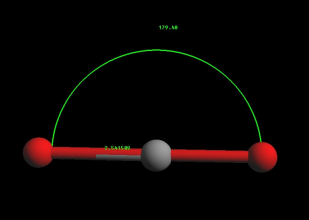
\includegraphics[width=8cm]{co2.png}
    \caption{Cząsteczka przed optymalizacją}
    \label{fig:co2}
  \end{figure}

  Rys. \ref{fig:co2uff} przedstawia model cząsteczki w którym wiązania \( C-O \) są
  pojedyncze - nie pozwala to na uzyskanie rzeczywistej geometrii.

  \begin{figure}[H]
    \centering
    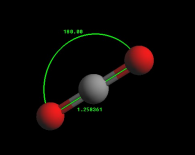
\includegraphics[width=8cm]{co2uff.png}
    \caption{Cząsteczka po optymalizacji UFF z wiązaniami pojedynczymi}
    \label{fig:co2uff}
  \end{figure}

  Rys. \ref{fig:co2uff2} przedstawia model cząsteczki z wiązaniami podwójnymi -
  uzyskana geometria jest w tym przypadku prawidłowa (dla użytej metody).

  \begin{figure}[H]
    \centering
    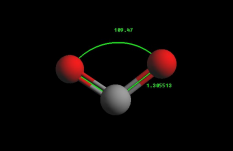
\includegraphics[width=8cm]{co2uff2.png}
    \caption{Cząsteczka po optymalizacji UFF z wiązaniami podwójnymi}
    \label{fig:co2uff2}
  \end{figure}

  Rys. \ref{fig:co2q} przedstawia cząsteczkę po optymalizacji metodą AM1, jest to
  metoda w której nie jest wymagane żadne wcześniejsze przygotowanie modelu.
  Geometria uzyskana metodami kwantowymi półempirycznymi przedstawia faktyczny
  układ atomów w cząsteczce.

  \begin{figure}[H]
    \centering
    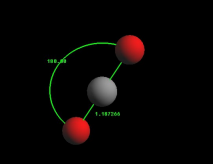
\includegraphics[width=8cm]{co2q.png}
    \caption{Cząsteczka po optymalizacji AM1}
    \label{fig:co2q}
  \end{figure}

  \subsection{Cząsteczka \( CH_2O \)}
  \begin{table}[h]
    \begin{adjustbox}{max width = \textwidth}
      \begin{tabular}{c|c|c|c|c}
      \textbf{Metoda}         & \textbf{Długość wiązania \( C-O \)\( [\angstrom] \)} & \textbf{Długość wiązania \( C-H \)\( [\angstrom] \)} & \textbf{Kąt \( H-C-H \)\( [^o] \)} & \textbf{Kąt \( H-C-O \)\( [^o] \)} \\ \hline
      UFF                     & 1,311214                                             & 1,336541                                             & 82,71                              & 130,94                             \\
      PM3                     & 1,201503                                             & 1,091525                                             & 116,54                             & 121,73                              
      \end{tabular}
    \end{adjustbox}
    \caption{Wyniki przedstawiające geometrię cząsteczki wg.\ użytych metod}
    \label{tab:wyniki_geomch2o}
  \end{table}
  \begin{table}[h]
    \begin{adjustbox}{max width = \textwidth}
      \begin{tabular}{c|c|c|c}
      \textbf{Metoda}         & \textbf{\begin{tabular}[c]{@{}c@{}}Energia całkowita\\ termodynamiczna\\ \( \left[\dfrac{kcal}{mol}\right] \)\end{tabular}} & \textbf{Ciepło tworzenia \( \left[\dfrac{kcal}{mol}\right] \)} & \textbf{Moment dipolowy \( [D] \)} \\ \hline
      UFF                     & 0                                                                                                                           & -                                                              & -                                  \\
      PM3                     & -10208,7036                                                                                                                 & -33,8951                                                       & 3,54530070                                 
      \end{tabular}
    \end{adjustbox}
    \caption{Wyniki przedstawiające właściwości fizyczne wg.\ użytych metod}
    \label{tab:wynikich2o}
  \end{table}

  Rys. \ref{fig:ch2ouff} przedstawia model cząsteczki \( CH_2O \) po optymalizacji
  metodą UFF

  \begin{figure}[H]
    \centering
    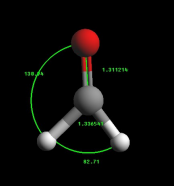
\includegraphics[width=8cm]{ch2ouff.png}
    \caption{Cząsteczka po optymalizacji UFF}
    \label{fig:ch2ouff}
  \end{figure}

  Rys. \ref{fig:ch2opm3} przedstawia model cząsteczki \( CH_2O \) po optymalizacji
  metodą PM3, możemy zaobserwować znaczącą poprawę dokładności rozmieszczenia atomów
  do ich rzeczywistej geometrii.

  \begin{figure}[H]
    \centering
    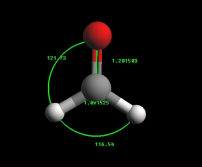
\includegraphics[width=8cm]{ch2opm3.png}
    \caption{Cząsteczka po optymalizacji PM3}
    \label{fig:ch2opm3}
  \end{figure}

  \section{Wnioski}
  Po wykonanych obliczeniach możemy stwierdzić, że metoda UFF, bez podania
  dodatkowych informacji takich jak informacja o rodzaju wiązań pomiędzy atomami
  daje niepoprawne wyniki. W przeciwieństwie do metody UFF, użyte metody kwantowe
  półempiryczne są znacznie szybsze, dokładniejsze i nie wymagają dodatkowych
  informacji wejściowych. Dobrze skonfigurowane metody klasyczne pozwalają uzyskać
  przybliżony obraz geometrii molekuły co pozwala na skrócenie czasu obliczeń kwantowych.

  \clearpage
  \begin{thebibliography}{9}
    \addcontentsline{toc}{section}{Bibliografia}
        
    \bibitem{arguslab}
    Obliczenia i wizualizacje zostały wykonane za pomocą:\\
    \textit{ArgusLab 4.0}\\
    Mark A. Thompson\\
    Planaria Software LLC, Seattle, WA.
    http://www.arguslab.com
  \end{thebibliography}

\end{document}